\documentclass[11pt]{report}

% French packages
\usepackage[utf8]{inputenc}
\usepackage[T1]{fontenc}
\usepackage[francais]{babel}

% Geometry
\usepackage[top=2cm, bottom=2cm, left=3cm, right=3cm]{geometry}

% Fonts
\usepackage{lmodern}

% Outline text
\usepackage{fancybox}

% Custom colors
\usepackage{xcolor}
    \definecolor{lightgray}{rgb}{.9,.9,.9}
    \definecolor{darkgray}{rgb}{.4,.4,.4}
    \definecolor{purple}{rgb}{0.65, 0.12, 0.82}

% Assets path
\usepackage{graphicx}
    \graphicspath{{./assets/}}

\usepackage{lipsum}
\usepackage{floatrow}

% Maths
\usepackage{amsmath}

\usepackage{tikz}
\usetikzlibrary{shapes,snakes}


\usepackage{multicol}

% Display code
\usepackage{listings}
    \definecolor{dkgreen}{rgb}{0,0.6,0}
    \definecolor{gray}{rgb}{0.5,0.5,0.5}
    \definecolor{mallow}{rgb}{0.58,0,0.82}

    % Captions style
    \renewcommand{\lstlistingname}{Source}

    % Listing list style
    \renewcommand\lstlistlistingname{Fichiers source}

    % Custom syntax highlighting
    \lstdefinelanguage{JavaScript}{
      keywords={typeof, new, true, false, catch, function, return, null, catch, switch, var, if, in, while, do, else, case, break class, let, const},
      ndkeywords={class, export, boolean, throw, implements, import, this},
      basicstyle=\ttfamily\scriptsize,
      sensitive=false,
      comment=[l]{//},
      morecomment=[s]{/*}{*/},
      morestring=[b]',
      morestring=[b]""
    }

    \lstset{
        language=JavaScript,
        aboveskip=3mm,
        belowskip=3mm,
        showstringspaces=false,
        columns=flexible,
        basicstyle={\small\ttfamily},
        numbers=none,
        numberstyle=\tiny\color{gray},
        keywordstyle=\color{blue},
        commentstyle=\color{dkgreen},
        stringstyle=\color{mallow},
        breaklines=true,
        breakatwhitespace=true,
        tabsize=4,
        frame=single
    }

% Header/footer
\usepackage{fancyhdr}
    \fancypagestyle{utt}{
        \setlength{\headheight}{23.96pt}
        \fancyfoot[C]{\thepage}
        \fancyhead[L]{\leftmark{}}
        \fancyhead[R]{
\includegraphics[scale=1.5]{logo_utt.jpg}}

        % Rename table of contents
        \addto\captionsfrench{\renewcommand{\contentsname}{Sommaire}}
    }

    \pagestyle{utt}

\title{Rapport - Travail d'investigation Technologique et Scientifique}
\author{Axel \bsc{Mousset} Aurélien \bsc{Labate} \\ Université de Technologie de Troyes}
\date{Printemps 2015}


\begin{document}
    \maketitle
    \chapter*{Remerciements}
    \pagenumbering{gobble}
    \noindent
    Merci à Alexandre Vial pour avoir bien voulu nous encadrer et croire en notre projet.\\
    Merci à Olivier Didon pour avoir réalisé les cartes électroniques du robot.\\
    Merci à Benoit Panicaud pour ses conseils en asservissement.\\
    Merci au club Robotik, pour son cadre de travail et son matériel.\\
    Merci au Bureau des étudiants, à l'institut des sports mécaniques et à l'administration pour leurs subventions.\\
    Et enfin merci à François [nom de famille] pour son usinage irréprochable de la mécanique.\\

    \pagenumbering{arabic}
    \tableofcontents

    \chapter{Introduction}
    L’objectif d’une TITS est de réaliser un projet avec un aspect scientifique de recherche, et une mise en application technique en découlant. La robotique, en tant que discipline hybride réunit parfaitement ces deux aspects tout en découpant sa dimension technique en un large spectre de compétences différentes : électroniques, informatiques et mécaniques, sans parler de management et de gestion de projet.\\

    Nous avons donc choisis de mener à bien le développement d’un robot. Les objectifs à remplir pour ce robot étaient sa parfaite autonomie, sa capaciter à pouvoir se repérer et se déplacer, et la gestion d’une pince mono-axe. Ce projet s’inscrit dans une dynamique associative : le robot réalisé a participé à la coupe de France de robotique, qui est un concours scientifique à l’échelle nationale réunissant plus de 200 équipes, sur lequel nous avons finit 54èmes. De plus comme notre association participe tous les ans à la Coupe, nous avons aussi souhaité faire en sorte que notre travail soit réutilisable. Ce projet a donc impliqué plus de quatres autres personnes régulièrement, étudiants, professeurs, et techniciens de l’UTT. Il est donc important de noter que ce document décrit l’essentiel de notre travail, à savoir électronique et informatique, mais aussi le projet dans sa globalité car il nous parait pertinent de replacer les réalisations dans leurs contexte.
    \chapter{Aspect général}
Le robot a pour objectif de pouvoir déplacer des objects cylindriques (cylindres en bois, et gobelets en plastique). Pour cela, nous l'avons équipé d'une pince adapté capable de monter et descendre.


\begin{figure}[h]
	\centering

	\begin{floatrow}
		\ffigbox[\FBwidth]{\caption{CAO du robot}}{%
			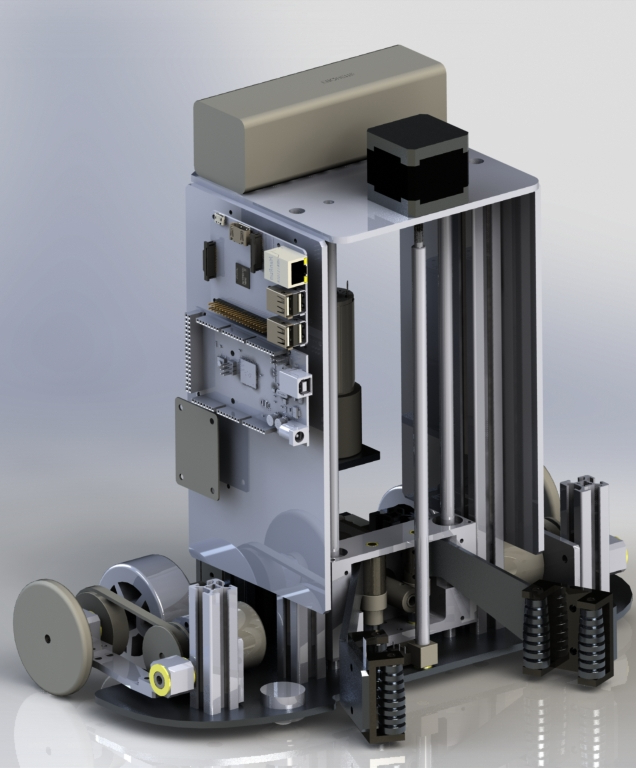
\includegraphics[width=70mm]{assets/3D-robot.jpg}%
		}
		\ffigbox[\FBwidth]{\caption{Photo du robot}}{%
			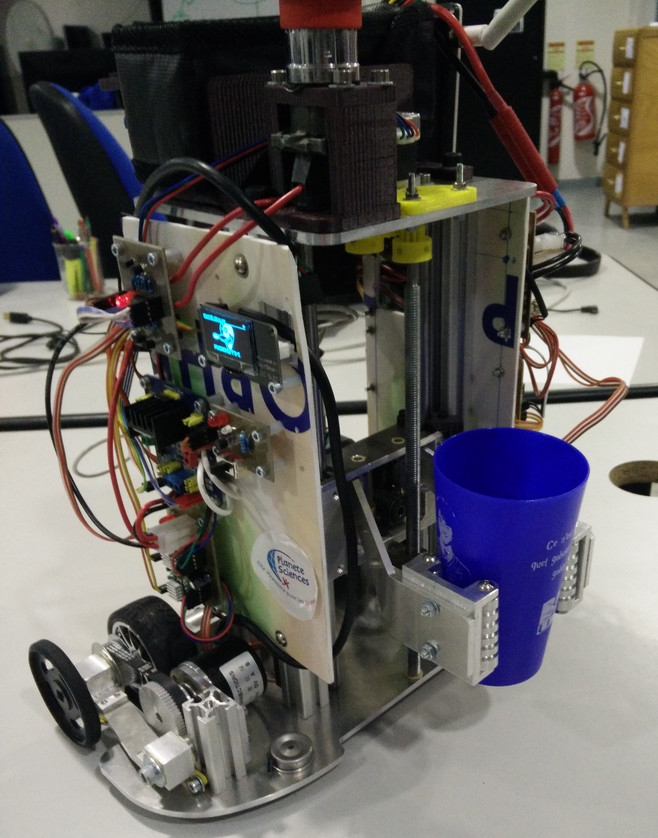
\includegraphics[width=70mm]{assets/photo-robot.jpg}%
		}
    \end{floatrow}
\end{figure}


\newpage
\section{Modularité}
Comme le club participe tous les ans à la coupe de France de Robotique, il y a des actions parfois similaire et certaines parties des robots qui pourraient être réutilisés. C'est en partant de ce constat que nous avons conçu une architecture modulaire. Certains modules pouvant être réutilisé et amélioré les années suivantes. \\


Cette année le robot a donc été séparé en 4 modules :

\begin{itemize}
	\item Coeur
	\item Moteur
	\item Pince 
	\item Capteur
\end{itemize}


\begin{figure}[h]
	\centering
	
% Define block styles
\tikzstyle{module} = [draw, text centered,text width=4em, minimum width=4em,
  minimum height=3.5em,ellipse]
\tikzstyle{object} = [draw, text centered, minimum width=2em,
  minimum height=1.5em]
\tikzstyle{arrow} = [thick, color=black!50, arrows=->, >=latex]
\tikzstyle{texto} = [above, text width=6em, text centered]

\begin{tikzpicture}[scale=0.675,transform shape]

%Modules
\node[module](A1) at (0,2){Coeur};
\node[module](A2) at (3,0){Module Pince};
\node[module](A3) at (0,-2){Module Capteur};
\node[module](A4) at (-3,0){Module Moteur};

%Bus I2C
\draw[arrow, <->] (A1.south) -- (A2.west);
\draw[arrow, <->] (A2.west) -- (A3.north);
\draw[arrow, <->] (A3.north) -- (A4.east);
\draw[arrow, <->] (A4.east) -- (A1.south);
\node[texto] at (0,-1.5ex){$I^2C$ Bus};

%Enfants de coeur
\node[object](B1) at (-2,3.5){Écran};
\node[object](B2) at (0,4.5){Sélection de couleur};
\node[object](B3) at (2,3.5){Lanceur};

\draw[arrow, ->] (A1.100) -- (B1.east);
\draw[arrow, <-] (A1.north) -- (B2.south);
\draw[arrow, <-] (A1.80) -- (B3.west);

%Enfant de moteur
\node[object, rounded corners](C1) at (-8.5,0.5){Contrôleur moteur à courant continu};
\node[object, rounded corners](C2) at (-8.5,-0.5){Carte acquisition roues codeuses};

\draw[arrow, ->] (A4.-190) -- (C1.east);
\draw[arrow, <-] (A4.-170) -- (C2.east);

	%Enfant de Controleur CC
	\node[object](D1) at (-10.25,2){Moteur gauche};
	\node[object](D2) at (-6.75,2){Moteur droit};
	
	\draw[arrow, ->] (C1.120) -- (D1.south);
	\draw[arrow, ->] (C1.100) -- (D2.south);

	%Enfant de acquisition roues codeuses
	\node[object](E1) at (-11,-2){Roue codeuse gauche};
	\node[object](E2) at (-6.75,-2){Roue codeuse droit};
	
	\draw[arrow, <-] (C2.-120) -- (E1.north);
	\draw[arrow, <-] (C2.-100) -- (E2.north);


%Enfants de Cpateur
\node[object](F1) at (-2.5,-3.25){Sonar 1};
\node[object](F2) at (-1,-4){Sonar 2};
\node[object](F3) at (1,-4){Sonar 3};
\node[object](F4) at (2.5,-3.25){Sonar 4};

\draw[arrow, <-] (A3.-120) -- (F1.east);
\draw[arrow, <-] (A3.-100) -- (F2.north);
\draw[arrow, <-] (A3.-80) -- (F3.north);
\draw[arrow, <-] (A3.-60) -- (F4.west);

%Enfant de pince
\node[object, rounded corners](G1) at (8,1){Contrôleur moteur pas à pas};
\node[object](G2) at (8,0){Capteur de fin d'ouverture};
\node[object](G3) at (8,-1){Capteur de fin d'ascension};

\draw[arrow, ->] (A2.20) -- (G1.west);
\draw[arrow, <-] (A2.0) -- (G2.west);
\draw[arrow, <-] (A2.-20) -- (G3.west);

	%Enfant de controleur de moteur pas à pas
	\node[object](G2) at (6,2.5){Moteur ascenseur};
	\node[object](G3) at (10,2.5){Moteur pince};

	\draw[arrow, ->] (G1.110) -- (G2.south);
	\draw[arrow, ->] (G1.70) -- (G3.south);

\end{tikzpicture}

	\caption{Structure des différents modules}
\end{figure}

\section{Programmes et documentation}
Afin de pouvoir travailler à plusieurs sur les programmes, nous utilisons \textit{Git}. C'est un logiciel qui est fait pour pouvoir fusionner des modifications sur les différents fichiers du projets tout en gardant un historique de toutes les modifications. Pour que ce logiciel fonctionne, il faut qu'il y ait un serveur qui stoque tous les codes sources aisi que l'historique de modification sur Internet.\\

Nous utilisons Github.com, qui est l'un des plus utilisé. Nous avons choisis de ne pas mettre notre code source en publique, car nous participons à une competition. Le fait de mettre en privé du code est payant sur Github.com, cependant nous avons fait la demande à Github d'accorder gratuitement des dépots\footnote{dépot: Sorte de dossier ou le code d'un projet y est placé}  privés gratuits en tant qu'association étudiante. Ils ont mis deux mois pour étudier la demande avant de l'accepter.\\

\newpage

Les programmes qui font fonctionner le robots suivent l'architecture modulaire. Nous avons donc créé les dépots suivants :\\
\begin{itemize}
	\item \textit{eurobot-core} : Le code du module Coeur
	\item \textit{eurobot-clampController} : Le code du module Pince
	\item \textit{eurobot-sensorController} : Le code du module Capteur
	\item \textit{eurobot-motorController} : Le code du module Moteur
	\item \textit{eurobot-CAO} : Les fichiers de conception 3D
	\item \textit{eurobot-debug} : Le code d'un script permettant d'afficher des informations utiles sur l'écran du robot
	\item \textit{eurobot-electronic} : Les fichiers de conception des cartes electroniques
\end{itemize}\ \\

Le projet du robot a aussi pour but de poser les bases d'une documentation interne pour le Club de Robotique. Ainsi en fin d'année dernière, nous avons mis en place un Wiki, c'est à dire une documentation où tout le monde peut participer (ici toutes les personnes du club).\\

Que ce soit le wiki ou le code et les fichiers placés sur github, elle resterons et permettrons aux équipes futurs d'avoir des connaissances et des examples sur lesquelles travailler. Ce qui nous avais cruellement manqué lorsque nous avons commencé.

\section{Electronique}
Le robot est alimenté par une batterie Lithium-Polymère de 4 cellulles et de 5000 mAh, ce qui veut dire qu'elle peut sort 14.8V et qu'elle peut délivrer jusqu'à 5A pendant une heure (ou 1A pendant 5 heures). \\

La batterie est branchée sur la carte de régulation qui permet permet principalement de réguler la tension de la batterie à 5V car la plupart de nos cartes fonctionnent à cette tension. Elle intègre aussi un interrupteur d'allumage général qui coupe la batterie et un bouton d'arret d'urgence qui coupe uniquement les moteurs. Un fusible y est aussi placé pour éviter d'endomager certaines cartes sensibles en cas de court-circuit. \\

Le robot dispose aussi d'une carte de conversion de tension 5V à 3,3V. La carte du module Coeur fonctionne en 3,3V alors que le reste du robot fonctionne en 5V. Cette carte permet donc de pouvoir communiquer entre les cartes sans que le module coeur soit endomagé par ine tension de 5V.


    \chapter{Coeur}

	Le coeur permet de contrôler les autres modules et donc les actions du robot. C'est l'intelligence artificielle du robot.


	\section{Specifications materiel}
	Le coeur est le module qui dispose du plus de puissance de calcul, de plus il doit pouvoir faire fonctionner un système linux tout en étant suffisament petit pour être embarqué dans le robot.\\

	Nous avons choisis d'utiliser une carte Odroid C1 avec un processeur quad-core pour 31,53 euros (35 dollars). Cependant avec les frais de port et de douane cette carte nous ait revenu à 52,53 euros.\\

	Cette année la Raspberry Pi 2 est sortie, elle concurrence l'Odroid C1 puisque, pour la même taille elle dispose elle aussi d'un processeur de puissance similaire. Cependant elle est sortie trop tard pour que nous l'utilisions cette année. Nous l'utiliserons sans doute l'année prochaine car elle est plus connue et on peut plus facilement résoudre des problèmes sur des cartes utilisés par plus de personnes.

	\section{Système d'exploitation}
	Nous allons utiliser un système Linux, car c'est plus adapté à nos besoins. Cependant il existe plusieurs versions (appelés distributions) différentes de ce système.\\

	Nous avons choisis d'utiliser la distribution \textbf{Archlinux} car il dispose des derniers logiciels créés pour les systèmes linux. Par exemple, \textit{SystemD}, un gestionnaire de service disponible sur archlinux depuis quelques années alors qu'il vient tous juste d'arriver d'autres distribution comme \textit{Debian}. De plus la comunauté Archlinux est très active et possède une documentation très utile.\\

	L'installation d'un système linux sur un robot, peut s'avéré dangereuse si on ne prend pas de précotions. Il arrive régulièremenet que le robot soit débranché sans éteindre normalement Linux, ce qui a parfois pour conséquence de corrompre le système de fichier. Plus d'une fois, il nous ait arrivé d'avoir un élément qui ne fonctionnait plus (par exemple : on ne peut plus se connecter au réseau Wifi généré par le robot). Cependant nous avions prévu une copie du disque système ce qui nous permettait de la refaire en 15min. Faire une image du disque système est vraiment nécéssaire, cette année l'UTC n'a pas participé à son premier match parce que leurs disque était corrompu et il a fallut plusieurs heures de réinstallation.\\

	Nous avons aussi réalisé divers document publié sur la documentation interne du club de robotique afin d'expliquer la procédure de configuration du système linux. Ainsi peut importe le support materiel, c'est assez rapide de configurer un nouveau système.

	\section{Language}
	L'avantage d'avoir un support avec de la puissance de calcul comme celui que l'on a, c'est qu'on peut se permettre d'utiliser des languages de programmation favorisant la rapidité de programmation et moins l'optimisation des calculs.\\

	Nous avons choisis d'utiliser, comme l'année dernière, le Javascript qui est executé avec NodeJS. C'est le même language qui est utilisé dans les navigateurs web afin d'avoir un contenu dynamique. Cependant, nous considérons ce language immature sur certains points, des mises à jour existent mais ne sont pas forcément facile à utiliser.\\

	La norme de javascript utilisé dans les navigateur et dans nodejs est appelé \textit{ECMAScript 5}. Nous avons choisis d'utiliser ECMAScript 6. Pour cela nous sommes passé par un transpiller, c'est à dire un logiciel qui va convertir notre code ES6 (ECMAScript 6) en code ES5. Cela ajoute malheureusement de la complexité dans le procéssus de programmation, bien qu'effectué automatiquement par des outils comme \textit{Gulp}.

	\section{Interface de gestion}
	Afin de pouvoir plus facilement travailler sur le robot, nous avons developpé des outils uniquement destinés aux tests et au développements. Ainsi nous avons un écran qui nous indique des informations comme les adresses IP du robot, ce qui nous permet de pouvoir facilement se connecter en réseau au robot.

	Nous avons aussi créé une interface accessible en navigateur qui permet de changer des constantes, activer des fonctionnaliter et controller des fonctionnalités du robot. Nous pouvons depuis cette interface controller les actions primaires du robot (faire tourner un moteur par exemple), mais aussi les actions plus complexes comme \"aller sur à un point du plateau\". L'interface dispose aussi d'autres outils comme des graphiques de suivis de l'orientation, ce qui nous permet d'étudier la façon dont le robot réagis à une consigne de mouvement. Par exemple si le robot fait beaucoup d'allers et retours avant de se stabiliser, nous le verrons sur le graphique.

	
	\begin{figure}
		\centering
		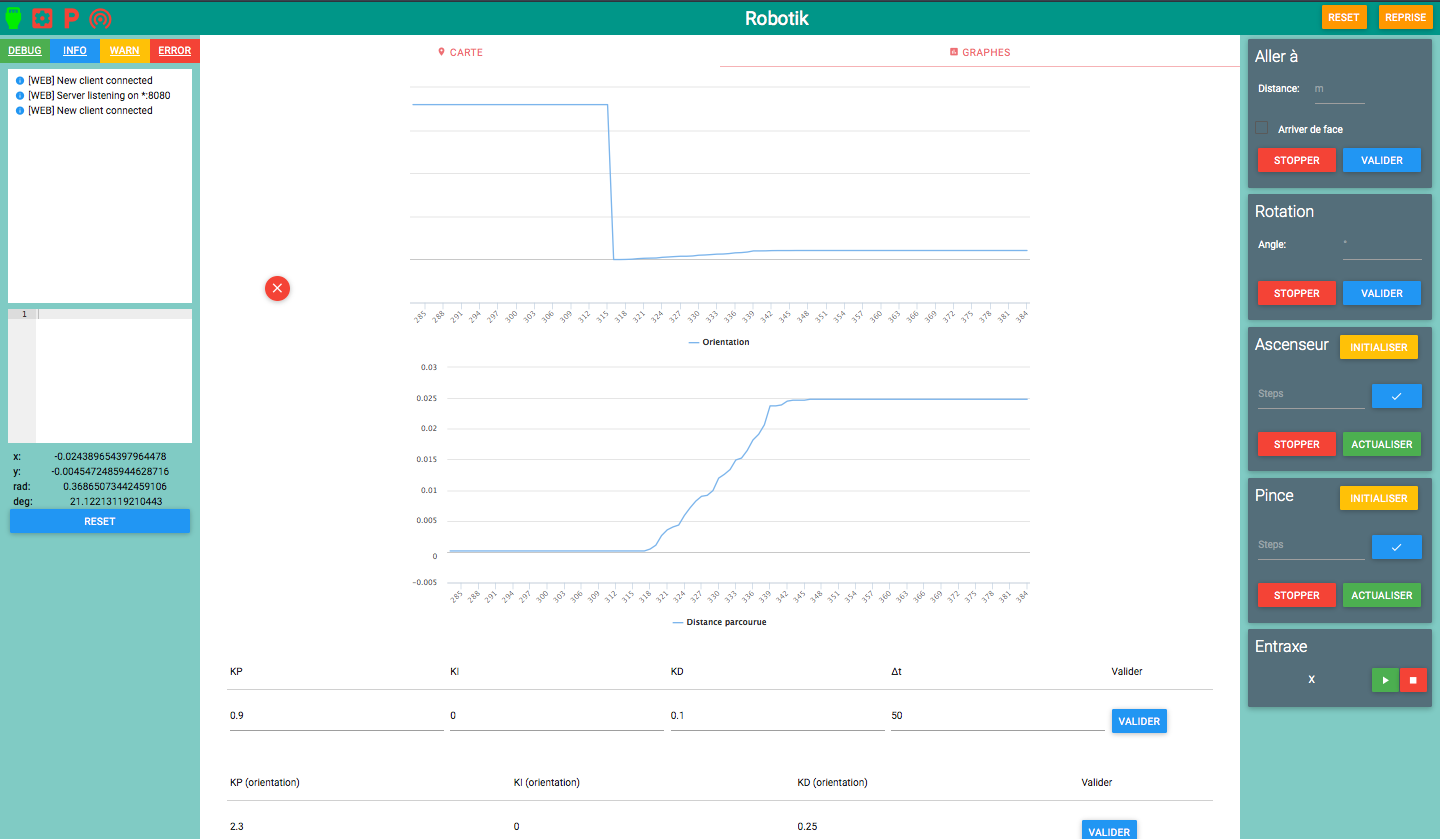
\includegraphics[width=150mm]{assets/debug.png}%
		\caption{Interface de gestion du robot}%
	\end{figure}


	\newpage

	\section{Ce qu'il faut améliorer}
	Sur ce module, nous sommes pour le moment assez satisfait de la puissance de calcul disponible et nous resterons donc sur le même type de support physique avec le même système d'exploitation poir l'année prochaine. Cependant il y a quelques points que l'on souhaite changer :

	\begin{itemize}
		\item \textbf{Une Raspberry Pi 2 au lieu d'une Odroid C1 :} Les différences entre ces deux cartes ne sont pas significatives, cependant, le support et la communauté est bien plus important sur la Raspberry Pi 2, ce qui lui assure une pérénité dans le projet : Si une personne reprend le club sans qu'il y ait de suivis, elle pourra plus facilement reprendre la même carte car elle la connaitra et qu'une simple recherche sur internet donne beaucoup d'informations. Ainsi le travail fait sur cette machine a plus de chance d'être réutilisé.
		\item \textbf{ECMAScript 6 vs ECMAScript 5 :} Cette année nous utilisions une norme pas encore supporté de notre language de programmation afin d'avoir certains avantages disponibles que dans la prochaine version. Cependant cela ajoutait beaucoup de complexité et nécéssite de configurer son système afin que le code soit transpilé juste pour devoir tester le code. L'année prochaine nous souhaitons baisser cette complexité. Et donc peut-être faire de l'ES5. Cependant, peut être que NodeJS (le logiciel qui execute notre code) disposera de nouvelles mises à jour qui lui permettrons d'executer un script javascript ES6.
		\item \textbf{Interface de gestion et simulateur :} Notre interface de gestion, bien qu'indispensable, pourrait être plus pratique, il est difficile de lui rajouter des fonctionnalité et elle n'est pas adapté à toutes les tailles d'écrans, en fait elle n'est pas adapté aux tailles d'écrans des developpeurs qui devaient dézoomer pour acceder à toutes les fonctionnalités. De plus on manque d'une interface de visualisation en 3D de ce que pense le robot qui pourrait être couplé à un simulateur.
	\end{itemize}
	On est plutot satisfait du travail sur ce module et nous comptons conserver une bonne partie du travail.
    \chapter{Esclaves}

Les 3 autres modules que Coeur sont dit \textit{esclaves} car ils n'envoient que des infos sommaires qui seront ensuite traitées par Coeur.

\section{Spécifications matérielles}
Chacun de ces 3 modules dispose d'une Arduino Nano dédié. Ce sont des petits microcontrôleurs se programmant en C++ et permettant de pouvoir manipuler des entrées et sorties logiques. Le fait d'en avoir trois séparés nous permet d'avoir des codes séparés et donc pouvoir isoler les problèmes et espérer une réutilisation de certains modules uniquement pour l'année suivante.\\

Afin de simplifier les branchements tout en pouvant facilement changer une Arduino qui aurrait été endommagée, nous avons fait une carte qui sert de support pour les Arduino Nano. Ainsi les arduino se branchent dans la carte comme on branche une prise.

\section{Communication}
Afin de faire communiquer les quatre modules entre eux, nous avons utilisé le protocole I2C. C'est un bus fonctionnant avec un maître et des esclaves. Le fait que ce soit un bus veut dire qu'avec deux fils de donnée, on peut brancher tous les modules entre eux et qu'on peut théoriquement en brancher plus d'une centaine sans que ça pose de problèmes. Le maître (ici core), est le seul à pouvoir parler et à demander aux autres de donner des informations. Un esclave ne peut pas donner des informations spontanément.\\

Nous avons ajouté des fonctionnalités à ce protocole afin d'éviter les erreurs de transmission et pouvoir faire en sorte que si le périphérique a des données disponibles, coeur lui demande de les donner. On a eu certains problèmes avec la communication, entre autres parce que le câblage était défaillant et qu'il suffisait d'un peu de mouvement pour avoir beaucoup d'erreurs.

\newpage
\section{Ce qu'il faut améliorer}
\subsection{La modularité}
Au niveau de la modularité, nous souhaitons pousser le concept plus loin au niveau de l'électronique. Ainsi, nous travaillons déjà avec un microcontrôleur par module, mais nous voudrions avoir réellement une carte complète électronique par module. Par exemple la carte de contrôle des moteurs embarquera :
\begin{itemize}
	\item Le microcontrôleur programmable (Arduino)
	\item La puce de contrôle des moteurs
	\item Le circuit d'acquisition des informations de roues codeuses
\end{itemize}
Alors qu'actuellement nous avons :
\begin{itemize}
	\item Une carte rassemblant les trois microcontrôleurs des trois modules
	\item Une carte contenant la puce de contrôle des moteurs
	\item Une carte contenant le circuit d'acquisition des informations de roues codeuses
\end{itemize}

\subsection{Le microcontrôleur programmable}


Pour des raisons de cout, nous souhaitons aussi faire nos propres arduino. Une arduino est principalement composé de 3 parties :

\begin{itemize}
	\item Un Atmega : C'est la base de l'arduino, celui qui éxecute le code. Cependant il ne coute que 3 ou 4 euros chez nos fournisseurs.
	\item Un régulateur de tension 5V : Inutile dans notre cas car nous avons déjà une tension régulée en 5V venant d'une carte de régulation.
	\item Un \"Convertisseur USB/Serial\" : Il permet de programmer et debugger l'arduino et coute très cher (15 euros pour celui de l'arduino Nano). Or nous n'en avons pas besoin d'un part arduino. De plus quand une arduino est endommagée, on perd ce module qu'on ne peut plus réutiliser pour une autre arduino, même si lui fonctionne bien.
\end{itemize}

Ainsi, l'année prochaine nous fabriquerons nos propres arduino et ne changerons que l'atmega s'il grille. Cela demande un peu plus de travail au niveau électronique mais c'est tout à fait faisable.

Au niveau de la communication, nous avons commencé nos recherches, et avons trouvé le protocole BUS CAN. C'est celui utilisé dans les voitures. Ses spécifications conviennent parfaitement à notre architecture. Le seul problème étant que ni l'arduino ni la Raspberry Pi ne le gère nativement. Cependant, il existe une puce permettant d'interfacer avec un bus CAN via spi, nous avons acheté des composants pour tester et nous ferons un prototype cet été pour voir si cette solution est viable.

\section{Le module pince}
Il s'occupe de gérer l'élévation de la pince et la fermeture de cette dernière.

\subsection{Mécanique}
La pince était actionnée par deux moteurs pas à pas et avait deux interrupteurs de fin de course afin d'initialiser les moteurs. La fermeture de la pince se passait bien. Par contre l'ascenseur de la pince était bien trop lent (30s pour monter). Nous avons ajouté un réducteur qui permet d'augmenter la vitesse par 5. Pour des raisons de rapidité de fabrication (ou de livraison), nous l'avons imprimé avec une imprimante 3D et il fonctionne comme escompté;.

La pince était faite pour acceuillir des éléments cylindrique ou conique et les empiler ce qui a plutot bien marché. Il fallait juste mettre des elastics pour ajouter de l'adhérence.

\subsection{Électronique}
Les contrôleurs moteurs que nous avons utilisés pour piloter les moteurs de la pince fonctionnent bien. Cependant la carte que nous avons fait ne prévoyait pas de pouvoir arrêter les contrôleurs moteurs, ce qui était une assez grosse erreur étant donné que les moteurs et les drivers chauffent constamment et par conduction, le châssis en alu devient lui aussi chaud. Nous avons mis des radiateurs sur les drivers, mais ce n'était pas suffisant. Lorsqu'on ne travaillait pas sur la pince, on était obligé de débrancher la carte ce qui est plutôt contraignant.

\subsection{Programmation}
Au début un algorithme permettant de faire des courbes trapezoidal avait été fait, cependant le temps de calcul était trop important pendant les mouvements de la pince et limitait la vitesse ce qui n'était pas négligeable sur l'ascenseur qui était déjà trop lent. L'algorithme a donc été simplifié et optimisé. Si le code était à refaire, il faudrait pouvoir détecter à tout moment les interrupteurs de fin de course, pouvoir facilement réactualiser la position à tout moment. Actuellement ils ne sont utilisés qu'à l'initialisation, quand les moteurs se calibrent.

\section{Le module capteur}
Il s'occupe de vérifier les sonars régulièrement pour voir s'il n'y a pas d'obstacle et s'il y a un obstacle, il prévient \textit{Core}.

\subsection{Positionnement des sonars}
Nous avions quatre sonars sur le robot :\\

\begin{itemize}
	\item Un devant en haut en biais
	\item Un derrière
	\item Deux en bas de chaque côté
\end{itemize}\ \\

Nous nous sommes vite rendu compte qu'il ne faut pas mettre de sonars en bas du robot car sinon ils détectent les éléments de jeu. Nous n'avons donc utilisé que le sonar en haut du robot car c'était le seul à ne pas les détecter.


\section{Le module moteur}
Ce module s'occupe de contrôler les déplacements et le positionnement du robot sur la table de jeu. Il utilise pour cela deux moteurs et deux roues codeuses. Ce module sera encore utilisé les années suivantes car nous avons besoin tous les ans d'un positionnement sur la table.

\subsection{Mécanique}
Afin d'avoir des roues codeuses séparées des moteurs, nous avons dû réduire la place que prenaient les moteurs. Le seul moyen en conservant ces moteurs était d'utiliser des renvois d'angles. Or avec les imperfections de réglage et d'usure; cela a créé des contraintes irrégulières sur le moteur ce qui les empêchait de tourner de façon régulière. En effet si on fixe le moteur et le renvoi d'angle sur le châssis et si l'arbre moteur est un peu tordu, il forcera à certains moments de la rotation. Cela a été l'un de nos plus gros problèmes pour asservir ces moteurs. Il est très difficile d'asservir le robot si les moteurs tournent de façon irrégulière.\\

Pour faciliter la rotation des moteurs, nous avons enlevé l'une des fixations : celle qui supportait l'axe de rotation des roues et donc l'arbre de sortie du renvoi d'angle. L'équipe mécanique a ensuite mis en place une bille folle à l'arrière du robot pour soulager les renvois d'angles. Cependant cela a été mis en place trop tard et à la coupe, ce qui a cassé, c'est le renvoi d'angle qui était bien trop affaibli. \\

Il faut simplifier la chaine de transmission l'année prochaine afin d'éviter ce genre de problème.

\subsection{Ce qu'il faut améliorer}
Cette année nous travaillons avec des moteurs à courant continue. Pour des raisons de place, nous souhaitons travailler l'année prochaine avec des moteurs brushless. Nous en avons retrouvé deux dans les armoires de Robotik et nous allons faire des tests cet été pour voir si on peut les contrôler comme on le souhaite avec les driver que nous a conseillé l'équipe de l'UTC.\\

Néanmoins le code et les connaissances ne sont pas perdus. C'est la partie du projet où nous avons investi le plus de temps, et c'est pourquoi nous avons choisi de développer plus en détail les algorithmes permettant de positionner le robot sur le plateau de jeu.
    \part{Algorithme}
\chapter{Odometrie}
    L’odometrie désigne l’évaluation de la position du robot dans un repère fixe à l’aide de
    mesures sur son déplacement. On se place dans le cas d’une odométrie calculée à l’aide de deux codeurs incrémentaux à quadrature montés sur roue codeuses. On distingue roues motrices et roues codeuses : en effet, disposer les codeurs directement sur l’arbre moteur risque de provoquer des enregistrement de déplacements liés à un patinage des moteurs en cas de roue motrice bloquée. Les methodes d’odometrie liés à l’utilisation de capteurs optiques ne seront pas traités ici.

    \section{contexte}
        On échantillonne les impulsions des encodeurs périodiquement tous les $d\tau$ . On choisit l’origine au millieu de l’essieu du robot, et on assimile le robot à ce point. La position du robot est représentée par le vecteur
        \begin{equation}
            p = \begin{pmatrix}
                x\\
                y\\
                \theta
            \end{pmatrix}
        \end{equation}

        Avec:
        \begin{itemize}
            \item $(x, y)$ La position du millieu de l’essieu
            \item $\theta$ L'orientation du robot
        \end{itemize}

    \newpage
    \section{Interprétation des signaux}
        \subsection{Valeur et sens de rotation}
        \begin{figure}[h]
            \begin{center}
                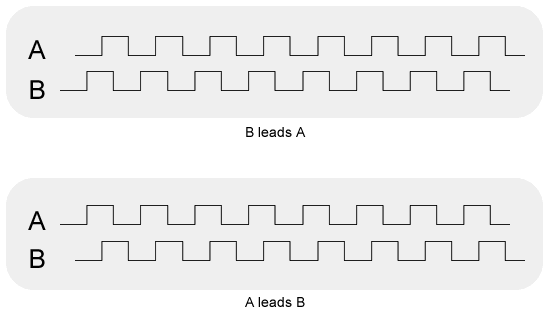
\includegraphics[scale=0.5]{encoder.png}
            \end{center}

            \caption{Signaux envoyés par un encodeur optique rotatif à quadrature}
        \end{figure}
        Chaque encodeur donne deux signaux : le signal A et le signal B. Chaque signal est déphasé de $\pi/4$, et le sens d’un signal peut être déduit de la valeur du deuxième signal au même moment.

        \textbf{Exemple} : l’écoute d’un front montant sur A peut être interpété comme une impulsion positive si l’état de B est à bas au même moment.\\
        On note :
        $$
            \begin{cases}
                impulsions_{gauche}\\
                impulsions_{droite}
            \end{cases}
        $$
        la \textit{somme algébrique des impulsions} depuis le dernier échantillonnage sur les roues gauche et droite.

        \subsubsection{Multiplication logicielle de la résolution}
            Il est possible de multiplier la résolution de son encodeur pour peu qu’il soit de bonne qualité, i.e que le rapport cyclique des signaux envoyés soit de 0.5. Notons que cette multipli-
            cation est purement logicielle, et que par conséquent elle induit une imprécision (bien qu’elle amène aussi une précision suplémentaire du au nombre d’impulsions plus important !).\\
            On peut ainsi doubler la résolution en comptant aussi bien les fronts montant que déscendant sur A, voir même quadrupler si on applique le même principe sur B.\\
            Dans le reste de ce document, on notera $C_r$ le coefficient de résolution, qui représente le nombre de fronts comptés par période du signal.

    \newpage
    \section{Formules de passage}
        On raisonnera la plupart du temps en impulsions d’encodeur et non en mètres. Voyons alors comment passer d’un système à un autre.\\
        On note :
        \begin{itemize}
            \item $impulsions_{parTour}$ le nombre d’impulsion d’encodeur par tour de roue codeuse.
            \item $impulsions_{codeur}$ le nombre d’impulsion d’un tour d’encodeur originel.
            \item $rapport_{reduction}$ le rapport de réduction entre le nombre de tour de roue codeuse et le nombre de tours d’encodeur.\\
        \end{itemize}

        On a la relation suivante :
        \begin{equation}
            impulsions_{parTour} = C_r \times rapport_{reduction} \times impulsion_{encodeur}
        \end{equation}
        Ainsi, pour passer de mètres en impulsions :
        \begin{equation}
            [m] = \frac{[impulsions] \times 2\pi \times R}{impulsions_{parTour}}
        \end{equation}

        \subsubsection{En pratique}
            On utilise le fait que la relation ci-dessus ne fait intervenir que des constantes.\\
            On peut donc la simplifier :
            \begin{equation}
                [m] = K_1 * [impulsions]
            \end{equation}
            Avec $K_1$ le facteur permettant de passer d’un système à l’autre. On le détermine alors empiriquement en faisant parcourir une distance $L$ en mètres au robot et on mesure la distance $\rho$ en impulsions parcourue. On trouve alors :
            \begin{equation}
                K_1 = \frac{L}{\rho}
            \end{equation}

    \newpage
    \section{Traitement des données}
        \begin{figure}[h]
            \begin{center}
                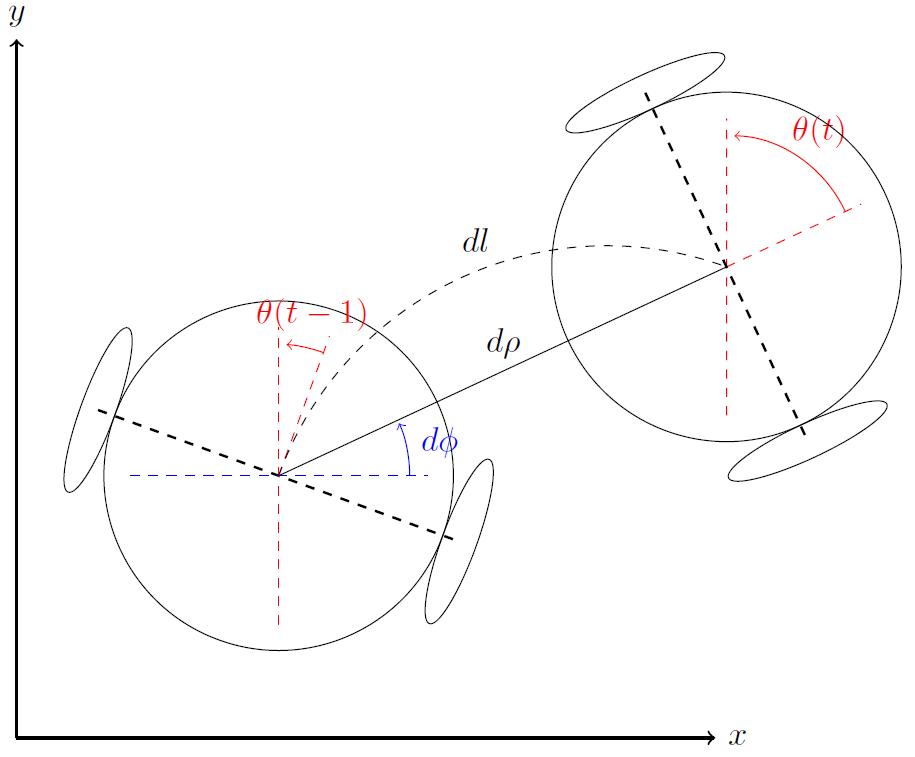
\includegraphics[scale=0.35]{odometry.png}
            \end{center}

            \caption{Evolution du système pendant $d\tau$}
        \end{figure}
        On fait une \textbf{approximation linéaire} sur le déplacement du robot, c’est à dire que l’on considère que sur un intervalle de temps $d\tau$ \textit{assez court} (en pratique 5ms semble suffisant), le déplacement dl du robot est une droite, i.e $d\rho$ = dl.\\
        De même, on consièdre que l’orientation de cette droite est la moyenne de l’orientation en début de déplacement et de l’orientation en fin de déplacement. On note alors $\phi$ l’angle de $d\rho$ :
        $$
            \phi = \frac{\theta(t) + \theta(t-1)}{2} = \theta(t-1)+ \frac{d\theta}{2}
        $$
        Au cours de $d\tau$ à l’instant t :
        \begin{equation}
            d\tau = \frac{impulsions_{gauche} + impulsions_{droite}}{2}
            \label{dTAU}
        \end{equation}
        \begin{equation}
            d\theta = \frac{impulsions_{gauche} - impulsions_{droite}}{entraxe}
            \label{dTHETA}
        \end{equation}
        Avec entraxe la distance entre le centre des deux roues codeuses.\\

        \textbf{En pratique} : Comme pour le facteur de passage entre ticks et mètres, la valeur de l’entraxe utilisée sur le système final doit être déterminée \textbf{empiriquement}. On fait alors tourner le robot sur $n\pi$ en sommant la différence de ticks. On trouve alors :
        \begin{equation}
            entraxe = \frac{\sum(impulsions_{gauche} - impulsions_{droite})}{n\pi}
        \end{equation}

        \newpage
        On procède à une intégration numérique\footnote{i.e une somme discrète, considérée continue car $d\tau$ est petit} pour obtenir l’orientation du robot dans le repère fixe:
        $$
            \theta(n) = \int_0^t d\theta
        $$
        Pour obtenir les coordonnées du robot dans le repère fixe, on projette la droite portée par $\rho$.
        \begin{equation}
            dx = d\rho \times cos(\theta(t-1) + \frac{d\theta}{2})
        \end{equation}
        \begin{equation}
            dy= d\tau \times sin(\theta(t-1) + \frac{d\theta}{2})
        \end{equation}
        A nouveaupar intégration numérique, on obtient les coordonnées du robot dans le repère fixe:
        $$ x(t) = \int_0^t dx $$
        $$ y(t) = \int_0^t dy $$
        Finalement, en notant $p$ la position du robot, on peut éxprimer $p'$ sa position après un échantillonnage.
        \begin{equation}
            p' =
            \begin{pmatrix}
                x\\
                y\\
                \theta
            \end{pmatrix} +
            \begin{pmatrix}
                \frac{impulsions_{gauche}+impoulsions_{droite}}{2}\times cos(\theta+\frac{impulsions_{gauche}-impulsions_{droite}}{2\times entraxe})\\
                \frac{impulsions_{gauche}+impoulsions_{droite}}{2}\times sin(\theta+\frac{impulsions_{gauche}-impulsions_{droite}}{2\times entraxe})\\
                \frac{impulsions_{gauche}-impulsions_{droite}}{entraxe}
            \end{pmatrix}
        \end{equation}

        \newpage
        \subsubsection{Code d'exemple}
            \begin{lstlisting}[language=JavaScript]
// Constantes theoriques
const REFRESH_TIME = 5; //ms
const RESOLUTION_COEF = 2;
const ENCODER_TICKS = 500;
const REDUCTOR_RATIO = 1.2;
const WHEEL_RADIUS = 0.06; //metres
const ENTRAXE = metersToTicks(0.5); //impulsions

let leftEncoder = new Encoder();
let rightEncoder = new Encoder();
let distance = 0;
let orientation = 0;
let x = 0;
let y = 0;
let lastCall = null;

function ticksToMeters(ticks) {
    return (ticks * 2 * Math.PI * WHEEL_RADIUS) /
        (RESOLUTION_COEF *REDUCTOR_RATIO * ENCODER_TICKS);
}

function metersToTicks(meters) {
    return (meters * RESOLUTION_COEF *REDUCTOR_RATIO * ENCODER_TICKS) /
        (2 * Math.PI * WHEEL_RADIUS);
}

/**
* Fonction de rafraichissement appelee le plus frequemment possible
*/
function compute() {
    let now = Date.now();
    // On s'assure que les calculs sont fait a intervalles reguliers
    if (now - previousOrientation >= REFRESH_TIME) {
        lastCall = now;
        let leftTicks = leftEncoder.getTicks();
        let rightTicks = leftEncoder.getTicks();
        leftEncoder.resetTicks();
        rightEncoder.resetTicks();
        let rho = (leftTicks + rightTicks) / 2;
        let dTheta = (leftTicks - rightTicks) / ENTRAXE;
        let dx = rho * Math.cos(orientation + dTheta / 2);
        let dy = rho * Math.sin(orientation + dTheta / 2);
        x += dx;
        y += dy;
        orientation += dTheta;
    }
}

function getRobotStatus() {
    return {
        x : ticksToMeters(x),
        y : ticksToMeters(y),
        orientation: orientation
    }
}
        \end{lstlisting}
    \chapter{Asservissement}
    Que ce soit en robotique ou dans différents processus industriels, il est souvent indispensable de contrôler certaines grandeurs physiques.
    On appelle \textbf{asservissement} d'une grandeur l'ensemble des moyens permettant de contrôler \textbf{automatiquement} cette grandeur.\\
    Celui-ci peut être mis en place soit au moyen d'un \textit{système en boucle ouverte}, c'est a dire en calculant une commande sans prendre en compte la réponse du système: le système nécessite alors une parfaite modélisation, nous ne nous attarderons donc pas sur ce type d'asservissement.\\
    L'asservissement dont nous allons parler se place dans le cas d'un \textbf{système en boucle fermée} ou \textbf{système à contre réaction négative}, qui, contrairement à son homologue ouvert, mesure la réaction du système pour adapter la commande. Toute la difficulté est alors de réussir à déterminer la fonction permettant d'adapter la commande de sortie en fonction de l'objectif voulu et du résultat mesurée.\\
    Le correcteur \textit{PID} est un exemple de système à boucle fermée permettant d'asservir efficacement une grandeur. C'est le correcteur le plus utlisié, qui a largement fait ses preuves dans l'industrie.
    \begin{figure}[h]
        \centering
        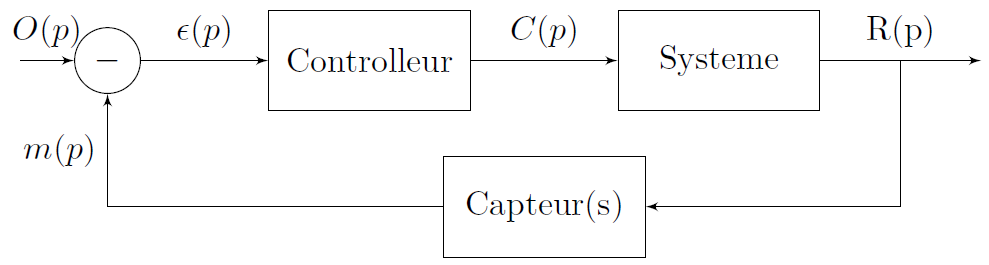
\includegraphics[scale=0.35]{assets/ASSERV.png}
        \caption{Représentation d'un système asservi en boucle fermée}
    \end{figure}


    \newpage
    \section{Correcteur PID}
        Le correcteur PID est un système à contre réaction \textbf{négative}, il calcule donc une commande en fonction de l'erreur $\epsilon$ de la grandeur, c'est à dire la différence entre la valeur voulue (i.e l'objectif) $O$, et valeur mesurée $m$.
        \begin{equation}
            \epsilon (t) = O(t) - m(t)
        \end{equation}
        La commande de sortie, passée au travers d'un correcteur PID, qu'on note $C(t)$, consiste en une somme de trois termes: une réponse proportionnelle à l'erreur, une réponse proportionnelle à la somme des erreurs, et une réponse proportionnelle à l'évolution de l'erreur. Une traduction quasi-litéralle de cette définition nous donne la relation suivante:
        \begin{equation}
            C(t) = f(\epsilon(t)) = K_p . \epsilon(t) + K_i . \int_{0}^{t}\epsilon(\tau).d\tau + K_d . \frac{d\epsilon}{dt}(t)
        \end{equation}
        Ou plus simplement\footnote{Les relations mettant en jeux des intégrales et des dérivées sont plus simples à exprimer dans le domaine de Laplace} dans le domaine de Laplace:
        \begin{equation}
            C(p) = f(\epsilon(p)) = K_p . \epsilon(p) + K_i . \frac{\epsilon(p)}{p} + K_d.p.\epsilon(p)
        \end{equation}
        Ce que l'on peut résumer à l'aide du schéma-bloc suivant:
        \begin{figure}[h]
            \centering
            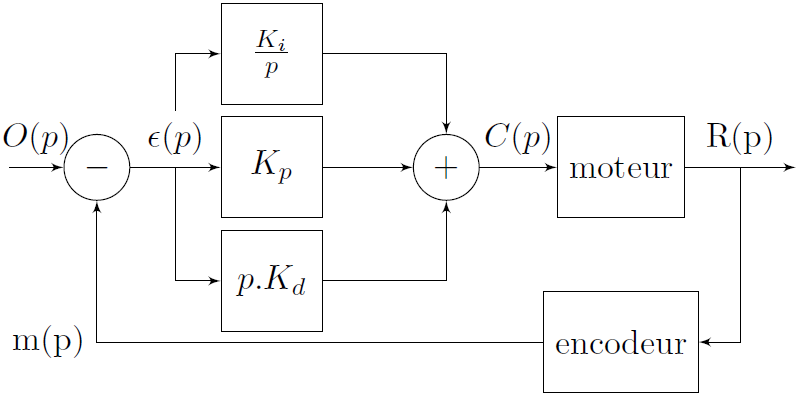
\includegraphics[scale=0.35]{assets/PID.png}
            \caption{Représentation d'un correcteur PID}
        \end{figure}

        \newpage
        \subsection{Influence des coefficients}
            Dans cette section, allons présenter l'influence des différents coefficients sur le système. En guise d'introduction à chacun d'eux, nous allons faire le parallèle avec un système (une voiture) et son correcteur pouvant être assimilé à un PID (un conducteur). On se place dans le cas ou sur une route, le conducteur décide d'être éxactement à la limite de la distance de sécurité de la voiture d'en face.

            \subsubsection{Réponse proportionnelle}
                \textit{«Plus je suis loin de la limite, plus je dois appuyer sur la pédale d'accélération.»}\\
                Le terme proportionnel permet de répondre aux grandes inerties du système, et diminue le temps de montée en donnant l'essentiel de la puissance au moteur: plus l'erreur est grande, plus la réponse est importante. La valeur de $K_p$ est proportionnelle à la vitesse de réaction du système. L'erreur statique est réduite avec l'augmentation de $K_p$, cependant le système perd en stabilité. En cas de $K_p$ démesuré, le système oscille et ne trouve jamais stabilité.\\
                Dans le cas d'un moteur, une variation trop faible de tension ne fait plus varier sa vitesse. Ainsi lorsque l'erreur devient trop faible, le terme proportionel ne permet pas de combler une erreur statique qui est d'autant plus faible que $K_p$ est grand.

            \subsubsection{Réponse intégrale}
                \textit{«Moins j'accélère pour une pression de la pédale d'accélération donnée, plus je dois appuyer sur la pédale.»}\\
                Le terme intégral fait la somme algébrique des erreurs. Il permet ainsi de donner une réponse de plus en plus forte à mesure que le système persiste dans son erreur. Il complète ainsi le terme proportionel, car permet de combler l'erreur statique laissée par ce dernier en régime permanent.\\
                Augementer $K_i$ permet de diminuer l'impact de faibles perturbations, augemente la précision du système en régime permanent. Un $K_i$ trop important peut cependant augementer le dépassement de la consigne «overshoot», et causer d'oscillations semblables à celles du $K_p$ en cas de valeur démesurée.

            \subsubsection{Réponse dérivée}
                \textit{«Plus j'accélère vite et que je me rapporoche de la limite (et risque donc de la dépasser), moins je dois appuyer sur la pédale.»}\\
                L'action du terme dérivé dépend du signe et de la vitesse de variation de l'erreur. Sa valeur va donc s'opposer à la réponse proportionnelle et intégrale. Elle devient importante lorsque l'erreur faiblit grandement et que le terme proportionnel continue à donner de grandes valeurs: elle freine le système empéchant le dépassement de la consigne et diminuant les petites oscillations qui ralentissent la stabilisation du système. $K_d$ compense donc $K_p$ lorsque l'erreur faiblit, on peut ainsi pousser $K_p$ pour limiter l'erreur statique quitte à dépasser la consigne, puis compenser ce dépassement en augementant $K_d$.

        \newpage

        \subsection{Réglage des coefficients}
            Régler les coefficients représente la majeure difficulté de la mise en place d'un asservissement PID. On s'intéresse ici uniquement à l'asservissement d'un moteur (à courant continu, ou pas).

            \subsubsection{Méthode théorique: Modélisation du système}
            Dans un premier temps, il est toujours intéressant de s'intéresser à la réponse théorique du système. Cette méthode n'est donc pas une méthode complète en soit, mais juste un outil permettant de "dégrossir" les coefficients avant de les affiner sur le système final.\\
            Les démonstrations des fonctions de transfert ci-dessous ne seront pas développées ici, car elle ne font pas l'objet de ce document. En effet, seul le modèle final et son utilisation nous intéresse.\\
            La fonction de transfert entre la vitesse angulaire de sortie et la tension d'entrée d'un moteur peut être modélisée comme un filtre du second ordre:
            \begin{equation}
                H(p) = \frac{\omega(p)}{U(p)} = \frac{A}{1 + \frac{2.\xi}{\omega_0} + \frac{1}{\omega_0^2}.p^2}
            \end{equation}
            Avec:
            \begin{itemize}
                \item $\omega(p)$ Vitesse de rotation du rotor
                \item $U(p)$ Tension appliquée au moteur
                \item $A = \frac{1}{K_e}$ Gain statique
                \item $\omega_0 = \sqrt{\frac{K_e.K_c}{L.J_T}}$ Pulsation propre
                \item $K_e/K_c$ Constante de vitesse/couple
                \item $J_T$ Moment d'inertie apporté au rotor
            \end{itemize}

            \paragraph{Moteur à courant continu}{
                \begin{itemize}
                    \item $\xi = \frac{R}{2}\sqrt{\frac{J_T}{K_e.K_c.L}}$ Facteur d'amortissement
                    \item $R$ Résistance au bornes du moteur
                    \item $L$ Inductance du moteur
                \end{itemize}
            }


            \paragraph{Moteur sans balais}{
                \begin{itemize}
                    \item $\xi = \frac{3R}{2}\sqrt{\frac{J_T}{K_e.K_c.L}}$ Facteur d'amortissement
                    \item $Ke = 0,0605.K_t$
                    \item $R$ Résistance phase-à-phase
                    \item $L$ Inductance phase-à-phase\\
                \end{itemize}
            }
            Il est possible de modéliser le moment d'inertie $J_T$ perçu par le moteur sur son arbre dans le cas d'une utilisation sur un robot de masse $M$ en connaissant le rayon des roues $R$.
            \begin{equation}
                J_T = M.R^2
            \end{equation}

            \newpage
            \subsubsection{Méthode empirique 1: dite de «Ziegler-Nichols»}
                La méthode de Ziegler-Nichols ne nécessite aucune modélisation au préalable, seule une batterie d'éssais expérimentaux souvent automatisables est nécessaire.\\
                Le principe est de fixer $K_i$ et $K_d$ à 0, puis d'augementer $K_p$ jusqu'à obtenir une réponse oscillante en régime permanent. On mesure alors la période $T_osc$ de cette réponse à $(K_p)_{lim}$.\\
                Les coefficients sont déduits de ces deux mesures par les relations suivantes:
                \begin{equation}
                \begin{cases}
                    K_p = 0.6 . (K_p)_{lim}\\
                    K_i = \frac{1}{0.5 . T}\\
                    K_d = 0.125 . T
                \end{cases}
                \end{equation}
                Les coefficients déduits sont assez polyvalents car ils proposent un bon compromis entre rapidité, dépassement de la consigne, stabilité, et précision. Néammoins, selon la spécification de la réponse désirée, il est possible d'ajuster les différents coefficients à la main. Par exemple, dans le cas de l'asservissement d'un robot, on va vouloir limiter au maximum le dépassement de consigne et donc baisser $K_p$.

            \subsubsection{Méthode empirique 2: dite «À la main»}
                Cette dernière méthode est utile lorsque l'on a des besoins spécifiques quant à la réponse du système. Par exemple, sur un asservissement en position, on peut vouloir complètement éliminer le dépassement de la consigne (il peut être critique d'aller trop loin et de déplacer un objet à la coupe de France !), quitte à avoir un temps de stabilisation plus long. Dans ce cas là, un asservissement de type PD est recommendable. Le principe est de faire varier $K_p$ jusqu'à qu'il y ai dépassement de consigne, puis de compenser en augmentant $K_d$ jusqu'à élimination de l'erreur statique.

    \section{Asservissement en vitesse}
        Première manière de contrôler le déplacement du robot: on asservit indépendemment chaque moteur en vitesse.\\
        Incovénient: pour aller à une position donnée, il faut donc intégrer numériquement les consignes de vitesse.
    \subsubsection{Code d'exemple}
            \begin{lstlisting}[language=JavaScript]
function velocityControl() {
    let velocity = encoder.getTicks(); // Vitesse en implusion par DeltaT
    encoder.resetTicks();

    previousVelocityError = velocityError;
    velocityError = velocityObjective - velocity;

    let derivative = velocityError - previousVelocityError; // On inclut le 1/DeltaT dans K_d
    integral += velocityError;

    velocityCommand = kp * velocityError + ki * integral + kd * derivative;

    return velocityCommand;
}
            \end{lstlisting}

    \newpage
    \section{Asservissement en position}
        Asservir indépendemment chaque moteur en position permet de résoudre le  problème d'intégration numérique. Par contre, la vitesse n'étant plus asservie, l'accélération peut être beaucoup trop grande, on s'expose alors à des risques de dérapages.
    \subsubsection{Code d'exemple}
            \begin{lstlisting}[language=JavaScript]
function positionControl() {
    position += encoder.getTicks(); // Position en ticks
    encoder.resetTicks();

    previousPositionError = positionError;
    positionError = velocityObjective - velocity;

    let derivative = positionError - previousPositionError; // On inclut le 1/DeltaT dans pKd
    integral += positionError;

    positionCommand = pKp * positionError + pKi * integral + pKd * derivative;

    return positionCommand;
}
            \end{lstlisting}

    \section{Asservissement en vitesse et en position}
        Réunir à la fois un asservissement en vitesse et en position permet de réunir le meilleur des deux mondes. On peut controller la vitesse, et donc l'accélération tout en se passant d'intégration numérique grace à l'asservissement en position.\\
        Un premier asservissement en position va donner une consigne de vitesse, qui après traitement algorithmique pour écrêter vitesse et accélération, va servir de consigne pour un deuxième asservissement en vitesse. On est donc capable de faire atteindre aux moteurs n'importe quelle position tout en controlant la vitesse ainsi que l'accélération à laquelle ils y vont.

        \subsubsection{Choix du profil de vitesse}
        Le profil de vitesse adopté est trapézoïdal. On commence par une phase d'accélération jusqu'à une vitesse de croisière, puis une déccélération jusqu'à atteindre la position voulue. L'avantage est de ne pas brusquer les moteurs, de ne pas déraper au démarrage et de ne pas dépasser l'objectif de position par inertie.

        \begin{figure}[h]
            \centering
            
\begin{tikzpicture}
% horizontal axis
\draw [->] (0,0) -- (8cm,0) node[below] {$t$};

% vertical axis
\draw[->] (0,0) -- (0,4cm) node[anchor=east] {$V$};

\foreach \x in {0,1,2,3,4, 5, 6, 7}
    \draw (\x cm,1pt) -- (\x cm,-1pt) node[anchor=north] {};
\foreach \y in {0,1,2,3}
    \draw (1pt,\y cm) -- (-1pt,\y cm) node[anchor=east] {};

% nominal speed
\draw[dotted] (2,0) -- (2,4);
\draw[dotted] (5,0) -- (5,4);

% Us
\draw[thick] (0,0) -- (2,2) -- (5,2) -- (7,0);
\draw (0.7,1.5) node {$A_{max}$}; %label
\draw (3.5,2.5) node {$V{max}$}; %label
\draw (6.3,1.5) node {$-A_{max}$}; 

\end{tikzpicture}
            \caption{Profil de vitesse trapézoïdal}
        \end{figure}

        \newpage

        Au niveau de l'algorithme, on tronque juste la valeur de la vitesse si elle dépasse une valeur $V_{max}$. On fait de même avec l'accélération en tronquant sa valeur absolue à $A_{max}$.
        \subsubsection{Code d'exemple}
            \begin{lstlisting}[language=JavaScript]
function motionControl() {
    previousVelocityObjective = positionCommand;
    velocityObjective = positionControl();

    // Ecretage de la vitesse
    if (Math.abs(velocityObjective) > maxVelocity) {
        velocityObjective = sign(velocityObjective) * maxVelocity;
    }

    let acceleration = velocityObjective - previousVelocityObjective;
    // Ecretage de l'acceleration
    if (Math.abs(acceleration) > maxAcceleration) {
        velocityObjective = previousVelocityObjective + sign(acceleration) * maxAcceleration;
    }

    motor.run(velocityControl());
}
            \end{lstlisting}

    \newpage
    \section{Asservissement polaire}
        Jusqu'à présent, tous les types d'asservissement proposés se faisaient sur une ou deux grandeurs, indépendemment sur chaque moteur. Il est possible de travailler sur des grandeurs «couplée», réunissant les informations fournies par les deux moteurs.\\

        Pour un robot, il peut être intéressant d'asservir sur la position et l'orientation. L'intérêt est de pouvoir facilement envoyer le robot à une une position $(x, y, \theta)$, sans avoir à faire du traitement algorithmique pour déterminer les consignes de position à envoyer à chaque moteur comme dans un asservissement position ou position/vitesse.\\
        On a donc en tout quatre controlleurs PID: deux pour un asservissement position/vitesse sur la vitesse de déplacement du robot, et deux pour un asservissement position/vitesse sur la vitesse angulaire du robot.\\
        Les grandeurs mesurées ne sont plus directement les impulsions d'encodeur, mais les variations de vitesse et de vitesse angulaire calculées par l'odométrie et décrites par les relations \eqref{dTAU} et \eqref{dTHETA} pour les PID de vitesse, et l'orientation/distance globale pour les PID de distance.

        \subsubsection{Code d'exemple}
            \begin{lstlisting}[language=JavaScript]
function robotControl() {
    /*
        Quadruple asservissement position/vitesse sur la distance et l'angle
        calcules par l'odometrie
    */
    let distanceVelocityCommand = distanceMotionControl();
    let orientationVelocityCommand = orientationMotionControl();

    /*
        Signe arbitraire. On part du principe que l'angle est calcule avec la
        difference entre la position gauche et droite
     */
    leftMotor.run(distanceVelocityCommand - orientationVelocityCommand);
    rightMotor.run(distanceVelocityCommand + orientationVelocityCommand);
}
            \end{lstlisting}

    \chapter{Conclusion}
    La réalisation du robot a été menée à son terme dans les délais que nous nous étions imposé pour concourrir à la coupe de France. Néanmoins, une casse de nature mécanique a empêché le robot d'être oppérationnel dès le premier jour. Ainsi, le robot secondaire (développé par d'autres étudiants) a quand même pu marquer des points.\\

    Malgré cet accident, ce projet nous a donné satisfaction. C'est en effet un réel projet d'ingénierie, alliant autant compétences scientifiques, techniques et humaines pendant plus de six mois d'efforts motivés par l'envie de performer dans une compétition.\\

    Au niveau personnel, l'ensemble des connaissances acquises est très enrichissant. Il a fallu effectuer un large travail documentaire en amont sur des sujets comme l'automatisation, l'asservissement ou encore l'odométrie. C'est donc avec passion que nous nous sommes attachés à mettre en pratique ces nouvelles connaissances aux côtés de celles apprises en cours pour réaliser ce robot.\\

    A un niveau plus large, nous éspérons que ce travail pourra répondre à l'une des problématique majeure dans le monde associatif à l'UTT, à savoir la transmission des savoirs. Le projet a donc largement été penser pour devenir potentiellement de base de référence pour futures années du club de robotique de l'UTT.

    \appendix
    \chapter{Suivi du projet}
    \begin{tabular}{|p{3cm}|c|p{10cm}|}
        \hline
        Personnes présentes & Date & Objet et synthèse\\
        \hline
        \hline
        Aurélien Labate, Axel Mousset, Alexandre Vial & 18/03/15 & Délimitation du sujet de TITS\\
        \hline
        Aurélien Labate, Axel Mousset, Alexandre Vial & 25/03/15 & Début du développement de l'interface de débug\\
        \hline
        Aurélien Labate, Axel Mousset, Alexandre Vial & 1/04/15 & Recherches documentaires sur Odométrie, Asservissement\\
        \hline
        Aurélien Labate, Axel Mousset, Alexandre Vial & 8/04/15 & Suite des recherches documentaires, premières discussions sur les solutions trouvées. Premier jet des cartes électroniques.\\
        \hline
        Aurélien Labate, Axel Mousset, Alexandre Vial & 15/04/15 & Fin des recherches. Développement des outils de simulation d'asservissement.\\
        \hline
        Aurélien Labate, Axel Mousset, Alexandre Vial & 22/04/15 & Développement du traceur de courbes pour pouvoir interpréter les réponses moteur.\\
        \hline
        Aurélien Labate, Axel Mousset, Alexandre Vial & 29/04/15 & Impression des cartes électroniques. Assemblage sur la mécanique et premiers tests d'asservissements polaire.\\
        \hline
        Aurélien Labate, Axel Mousset, Alexandre Vial & 6/05/15 & Mise au point, harmonistation des différents modules et préparation du départ à la coupe de France.\\
        \hline
        Annulé & 13/05/15 & \textbf{Coupe de France de robotique}\\
        \hline
        Aurélien Labate, Axel Mousset, Alexandre Vial & 20/05/15 & Lol\\
        \hline
        Aurélien Labate, Axel Mousset, Alexandre Vial & 27/05/15 & Lol\\
        \hline
        Aurélien Labate, Axel Mousset, Alexandre Vial & 3/06/15 & Lol\\
        \hline
     \end{tabular}


\newpage
\chapter{Memento sur les influences des coefficients PID}

    \nocite{*}
    \bibliographystyle{plain-fr}
    \bibliography{references}
\end{document}